\section{\Large PROBLEM SET 5}
\subsection{PROBLEM 1}
\textit{Gravity gradient torque (stability)}

\textit{a. Calculate the coefficients Ki of the moments of inertia which drive stability under gravity gradient. Compute and plot regions of stable and unstable motion similar to the picture below:}

The following equations show the relationships for gravity gradient stability in terms of moments of inertia.

% Insert equations for kR and kT as well as moment of inertia inequalities from lecture 8

We show the plot of stable and unstable motion under gravity gradient. When computing the coefficients using moments of inertia about the principal axes, we obtain the following plot.

\begin{figure}[H]
\centering
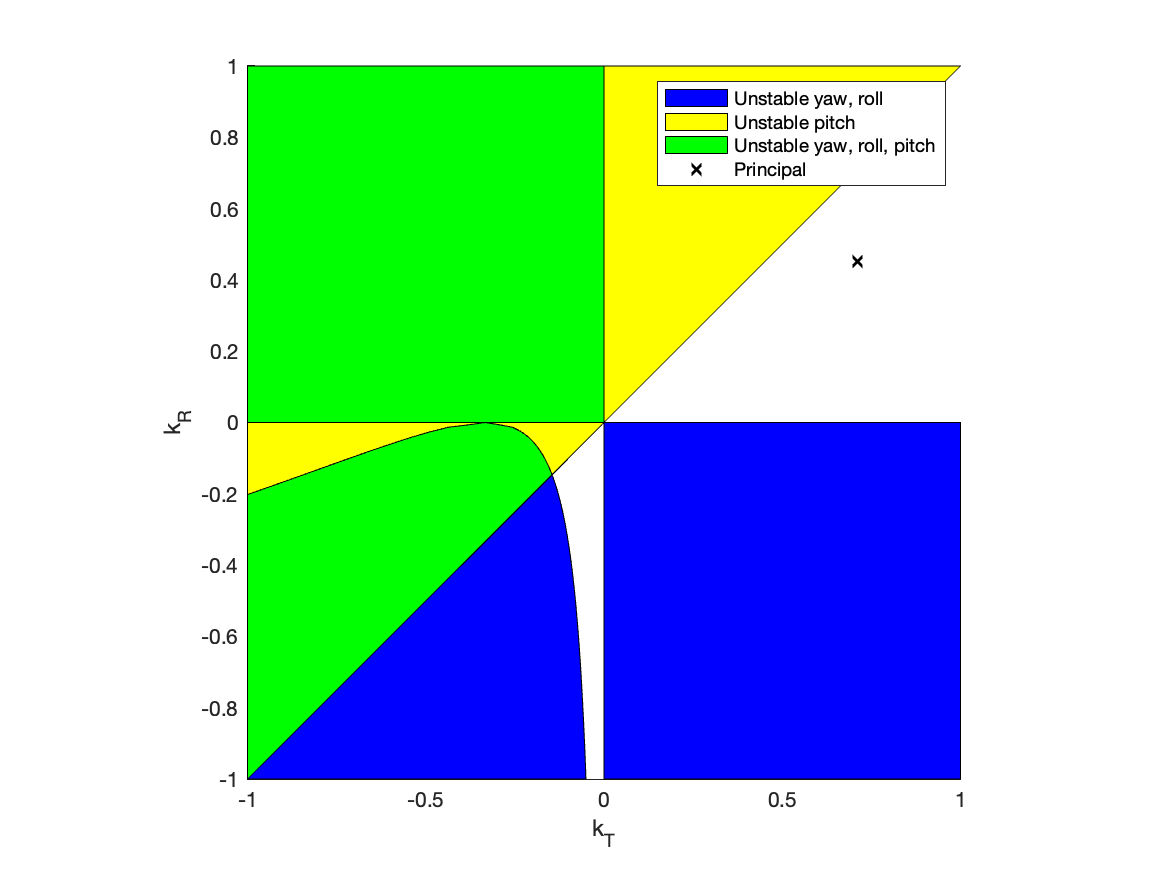
\includegraphics[scale=0.6]{Images/ps5_problem1a.png}
\caption{Stability for principal axes}
\label{fig:ps5_problem1a}
\end{figure}

\textit{b. Considering the results from 1a, comments on the expected stability of the attitude motion of your satellite about equilibrium. Try to reproduce stable and unstable motion by setting proper initial conditions and perturbing those conditions slightly (e.g., by 1\%). Plot attitude parameters (e.g., Euler angles) to show stability or instability.}

We expect stable behavior for small perturbations. Previously, we have already shown that aligning principal axes with RTN produces stable behavior when there are no perturbations. Now, we will introduce small perturbations.

\begin{figure}[H]
\centering
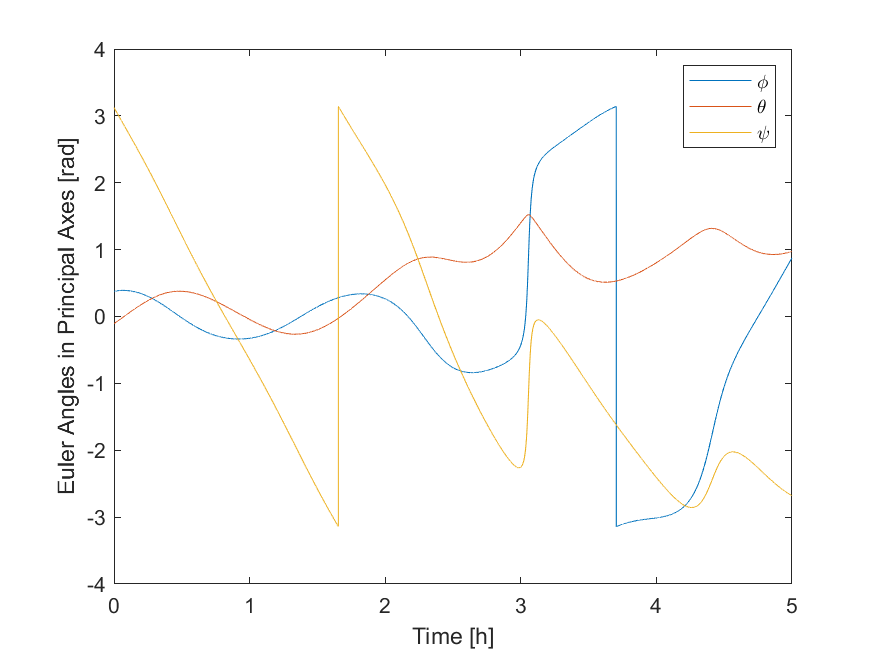
\includegraphics[scale=0.6]{Images/ps5_problem1b_angle.png}
\caption{Attitude evolution for stable orientation with 1\% perturbations}
\label{fig:ps5_problem1b_angle}
\end{figure}

\begin{figure}[H]
\centering
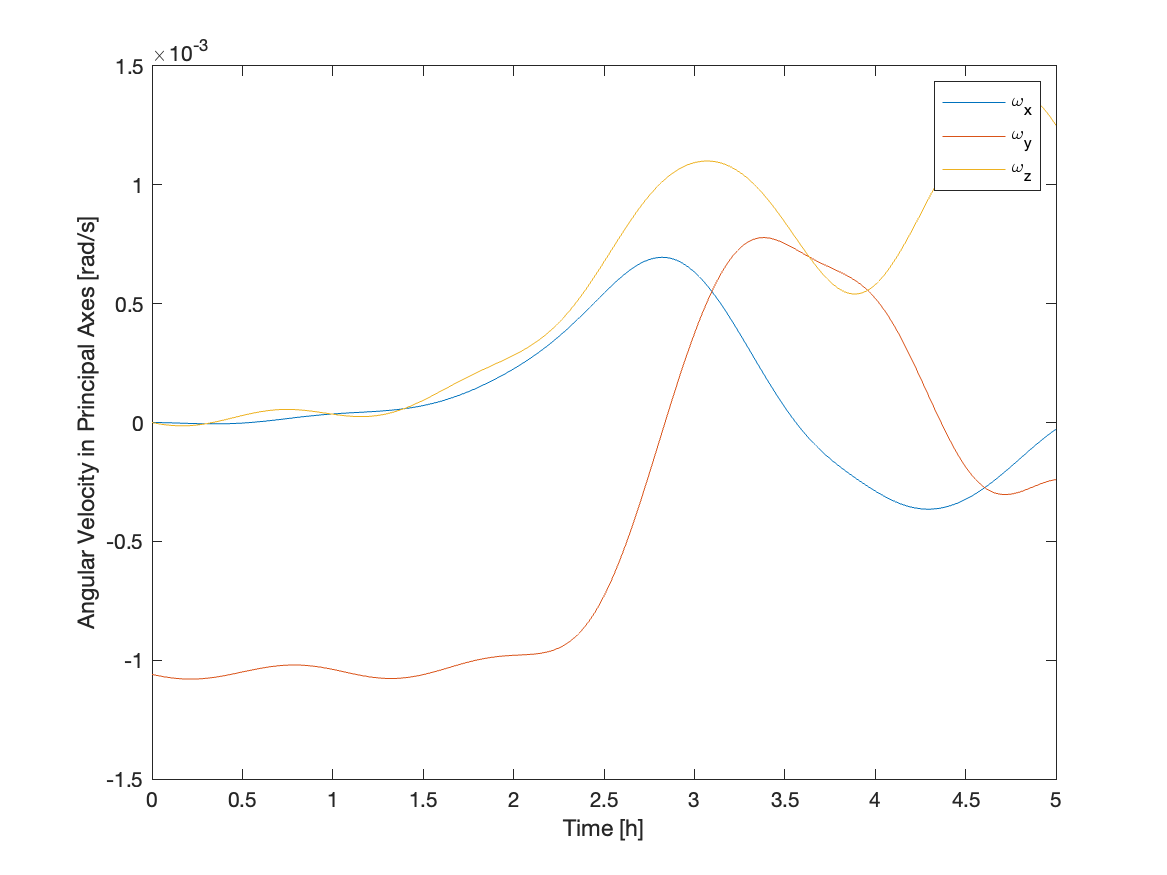
\includegraphics[scale=0.6]{Images/ps5_problem1b_angvel.png}
\caption{Angular velocity evolution for stable orientation with 1\% perturbations}
\label{fig:ps5_problem1b_angvel}
\end{figure}

As expected, our attitude motion (angular velocities and Euler angles) are periodically stable with a small perturbation in initial condition.


\textit{c. How would you need to change the mass distribution and/or nominal attitude of your satellite to obtain stable motion from the gravity gradient torque? Would it make sense for your project? Show a couple of potential configurations in the Ki plane and resulting stability of attitude motion at the equilibrium. This is done by changing your inertia tensor and simulating numerically.}

While we have already shown that the existing mass distribution is stable for gravity gradient torque, we investigate the stability for the satellite when it is rotated such that the spacecraft is oriented appropriately for SAR operations, that is, body x-axis is cross-track, body y-axis is along-track, and body z-axis is radial. However, this orientation is unstable, as shown in part (e) of Section 4.4.

\begin{figure}[H]
\centering
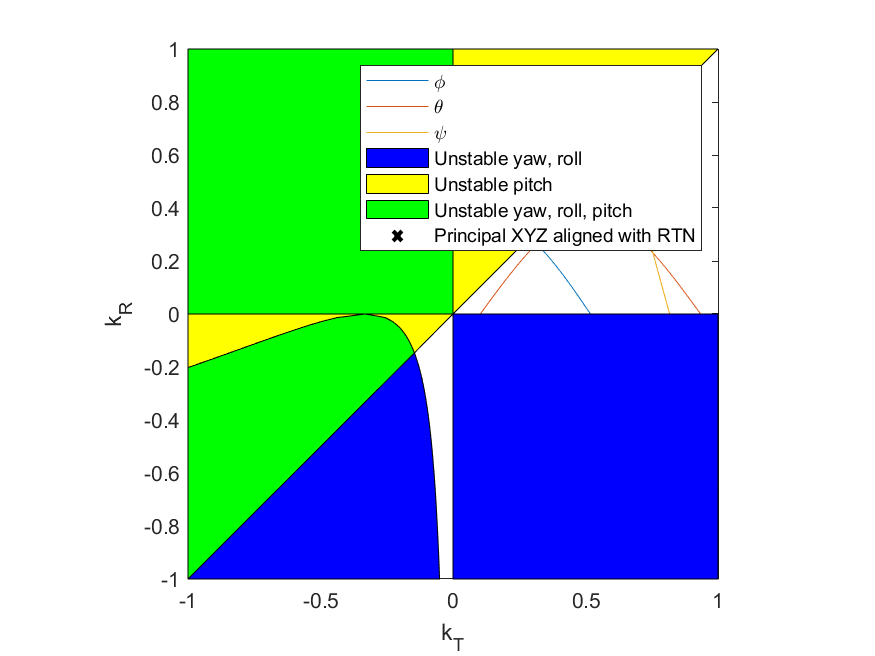
\includegraphics[scale=0.6]{Images/ps5_problem1c.png}
\caption{Stability for body axes}
\label{fig:ps5_problem1c}
\end{figure}

We must maintain this orientation in order to properly point the radar antenna located at the top of the spacecraft, so it does not make sense to orient the satellite along principal axes for gravity gradient stability. Instead, we will likely require magnetorquers to offset angular momentum changes from environmental torques.


\subsection{PROBLEM 2}
\textit{In addition to gravity gradient, start programming perturbation torques due to magnetic field, solar radiation pressure, and atmospheric drag. Note 1: You should apply a very minimal/basic model for perturbations that are not relevant (negligible) to your project. It is expected that you do not ignore them. Note 2: All perturbations can be grouped into a single large subsystem called environment or similar whose output feed
the Euler equations. Note 3: Re-use as many functions as possible for solar radiation pressure and atmospheric drag.}

The following function enables the propagation of the orbit with the specified perturbation torques.

\lstinputlisting{src/orbitTorque.m}

\subsection{PROBLEM 3}
\textit{Include all torques you have been able to model in numerical integration. Please show comparison of numerically computed disturbance torques with expected values and trend from theory (model) and tables (Wertz) referenced in class. Plot all torque components in principal axes over time. Plot the resultant (sum) of all torques in principal axes. Make sure that your model is not too ideal, i.e. make sure that center of pressure and center of mass do not coincide.}

